\chapter{Аналитический раздел}
\label{cha:analysis}

\section{Анализ решений}

Диаграмма деятельности ~--- это, по существу, блок-схема, которая показывает, как поток управления переходит от одной деятельности к другой, при этом внимание фиксируется на результате деятельности. Результат может привести к изменению состояния системы или возвращению некоторого значения. Она отличается от традиционной блок-схемы более высоким уровнем абстракции, возможностью представления с помощью диаграмм деятельности управления параллельными потоками наряду с последовательным управлением.

Обычную блок-схему можно представить в виде конечного автомата, так как в любой момент времени из одной вершины поток выполнения переходит строго в одну другую. Теория автоматов имеет широкое распространение и для них реализовано множество методов, что делает задачу анализа весьма тривиальной задачей. Но с помощью автомата нельзя представить схемы с параллельными вычислениями, поэтому возникает необходимость использовать другой математический аппарат для исследования их поведения.

Таким аппаратом стали сети Петри, созданные специально для моделирования дискретных динамических систем. Сеть Петри представляет собой двудольный ориентированный граф, состоящий из вершин двух типов — позиций и переходов, соединённых между собой дугами. Вершины одного типа не могут быть соединены непосредственно. В позициях могут размещаться метки (маркеры), способные перемещаться по сети. Для анализа сетей Петри существует два метода: матричный метод и метод построения дерева достижимости. Оба метода имеют свои недостатки, но, применимо к данной проблематике лучшие результаты будет давать метод, основанный на дереьях достижимости.

\section{Обзор существующих решений}

\subsection{CPN Tools}

CPN Tools ~--- это специальная моделирующая система, которая использует язык сетей Петри для описания моделей. Система была разработана в Университете Орхуса в Дании и свободно распространяется для некоммерческих организаций (http://cpntools.org/). CPN Tools предлагает очень мощный класс сетей Петри для описания моделей. Согласно стандартной классификации такие сети называют иерархическими временными раскрашенными сетями Петри. Было доказано, что они эквивалентны машине Тьюринга и составляет универсальную алгоритмическую систему. Таким образом, произвольный объект может быть описан с помощью этого класса сетей.

Простейшая концепция раскрашенной сети Петри использует различные типы фишек, где тип фишки определен натуральным числом и визуально представлен как цвет. Концепция раскрашенной сети Петри CPN Tools более сложная. Такие сети часто называют обобщенными раскрашенными сетями, так как тип фишки представлен абстрактным типом данных, как в языках программирования. Термин «раскрашенная» сохраняется исторически, но теперь очень трудно представить такие «цвета» визуально.

Временные сети Петри используют понятие модельного времени для описания продолжительности действий в реальных объектах. В отличие от классических сетей Петри, где срабатывание перехода происходит мгновенно, срабатывание перехода во временной сети связано с определенной продолжительностью или временной задержкой. Это позволяет анализировать временные характеристики реальных объектов, например, время отклика как характеристику качества обслуживания сети.

Иерархические сети обеспечивают построение сложных моделей. В таких сетях элемент может быть представлен другой сетью. В CPN Tools переход может быть замещен дополнительной сетью. Таким образом, получается вложенная конструкция: сеть внутри сети. Количество уровней иерархии не имеет принципиальных ограничений. Отметим, что, такой подход широко распространен в языках программирования, где процедуры используются для управления сложностью.

Для достаточно простых моделей возможна генерация полного пространства состояний (графа достижимости). Это ~--- лучший способ для верификации, например, телекоммуникационных протоколов. CPN Tools обеспечивает построение пространства состояний и автоматическую генерацию по нему отчёта, который содержит выводы о стандартных свойствах сетей Петри, таких как ограниченность и живость. Кроме того, предусмотрен специальный язык на основе языка CPN ML для описания запросов о
нестандартных свойствах пространства состояний, которые важны для пользователя. К сожалению, для сложных моделей пространство состояний может быть слишком большим, и его построение не представляется возможным.

Единственный способ для анализа сложных моделей ~--- это имитация их поведения. CPN Tools предусматривает пошаговую имитацию для поиска и устранения ошибок в разрабатываемой модели, а также автоматическое выполнение определенного количества шагов. Имитация на больших временных интервалах – это путь для статистического анализа поведения модели. Такой подход применяется для оценки характеристик телекоммуникационных сетей, например, пропускной способности и качества обслуживания.

\subsection{UniMod}

UniMod является разработкой кафедры компьютерных технологий Санкт-Питербургского университета информационных технологий, механики и оптики. Долгосрочная цель проекта заключается в создании единой методологии для разработки и дальнейшего развития, что позволит сократить разрыв между проектированием и разработкой.

Проект UniMod (http://unimod.sourceforge.net) с открытым исходным кодом содержит набор инструментов, позволяющих визуально проектировать и реализовывать программы. При этом первоначально строится схема связей, состоящая, как и в \textit{switch-технологии}, из источников событий, системы управления и объектов управления, в которых реализованы вызываемые из автоматов выходные воздействия и опрашиваемые автоматами входные переменные. В данном случае система управления ~--- это система взаимосвязанных автоматов.

Такой подход к проектированию систем акцентирует внимание разработчиков на изучении предметной области, выделении объектов управления и поставщиков событий. Затем проектируется один или несколько автоматов, для каждого из которых создается схема связей и граф переходов. Такой подход позволяет на ранних стадиях проектирования выявить и устранить множество возникающих неясностей в постановке задачи, а также предусмотреть весьма не очевидные детали поведения системы.

Сначала формируются события, обрабатываемые одним из автоматов в соответствии с графом переходов. Автомат при поступлении события может проверить различные логические условия и в результате выбрать необходимый переход в новое состояние. С переходом может быть ассоциирован некий набор выходных воздействий на объекты управления. Эти воздействия выполняются при выборе данного перехода. В общем случае действия могут выполняться не только на переходах. При поступлении определенного события автомат может перейти в конечное состояние, завершив тем самым работу приложения.

Одна из сильных сторон пакета UniMod ~--- это возможность визуального конструирования программ. В отличие от распространенного подхода, когда вспомогательные картинки и UML-диаграммы рисуются с надеждой на улучшение документации и продуктивности труда, разработанные с помощью инструментального средства UniMod диаграммы и вручную написанные классы в целом формируют работающее приложение.

\subsection{Язык программирования ДРАКОН}

Наиболее близким и точным аналогом диаграмм деятельности являются математически строгие дракон-схемы визуального алгоритмического языка ДРАКОН. Более отдаленным аналогом являются схемы алгоритмов по ГОСТ 19.701-90.

ДРАКОН (Дружелюбный Русский Алгоритмический язык, Который Обеспечивает Наглядность) ~--- визуальный алгоритмический язык программирования. Был разработан в рамках космической программы «Буран». Основной задачей разработчиков было создание единого универсального языка программирования, который своей доступностью и мощностью был бы способен заменить специализированные языки ПРОЛ2 (для разработки бортовых комплексных программ Бурана), ДИПОЛЬ (для создания наземных программ Бурана) и ЛАКС (для моделирования). В качестве аксиоматики для ДРАКОНа были выбраны устремлённые графы (специальный класс циклических орграфов). Такое двумерное структурное программирование годится для доказательного построения алгоритмов методом Дейкстры. В отличие от блок-схем, дракон-схемы имеют средства для описания работы в реальном времени.

Некоторые ученые считают, что существующие способы записи алгоритмов и программ (принятые во всем мире) слишком трудны для понимания и требуют неоправданно больших трудозатрат. Это обстоятельство ставит непреодолимый барьер для многих специалистов, работа которых связана с алгоритмами, но которые не имеют резерва времени, чтобы научиться выражать свои профессиональные знания в форме алгоритмов и программ. Язык ДРАКОН использует новую эргономичную нотацию (дракон-схемы) и за счет этого существенно облегчает алгоритмизацию и программирование. Благодаря использованию дракон-схем алгоритмы и программы становятся более понятными, доходчивыми, ясными, прозрачными.

ДРАКОН ~--- графический (визуальный) язык, в котором используются два типа элементов:
\begin{itemize}
\item графические фигуры (иконы);
\item текстовые надписи, расположенные внутри или снаружи икон (текстоэлементы).
\end{itemize}

Поэтому язык ДРАКОН имеет не один, а два синтаксиса: графический и текстовый.
Графический (визуальный) синтаксис охватывает алфавит икон, правила их размещения в поле чертежа и правила связи икон с помощью соединительных линий. Текстовый синтаксис задает алфавит символов, правила их комбинирования и привязку к иконам. (Привязка необходима потому, что внутри разных икон используются разные типы выражений). Императивная (процедурная) часть языка Дракон может описываеться на основных языках программирования (c, c\#, pascal и т.д.)

Cистема получается как результат процедурной декомпозиции деятельности на два и более алгопроцессов связанных отношением вызова и/или взаимодействия, т.е. решение сложной задачи мы разбиваем на подзадачи. В алгоритме решения при этом выделяем основной алгоритм и вспомогательные («вставки» в терминах языка ДРАКОН).

ДРАКОН поддерживает декомпозицию алгоритма выделением вспомогательных алгоритмов-вставок («предопределённых процессов» в терминах блок-схем по ГОСТ 19.701-90).

Представляемые схемами модели процессы могут находиться либо в отношении «главный-подчинённый» (иерархическая, или ранговая модель), либо в отношении «партнёров» (одноранговая, или диспозитивная модель). По порядку же возникновения всегда существует первичный процесс, который для другого данного процесса бывает:
\begin{itemize}
\item вызывающий ~--- когда данный процесс был вставкой (во вставку во вставку и т. д. ~--- если уровней вызова много) в другой процесс;
\item «родительский» ~--- когда данный процесс порождён как часть системы т. н. совместно протекающих взаимодействующих процессов (асинхронных или параллельных).
\end{itemize}

В ранговой модели существует только одна рабочая точка. Она последовательно проходит процессы, начиная с первичного вызывающего. Там, где указана вставка другого процесса, совершается переход на его схему. Когда эта схема пройдена до конца ~--- переход обратно на место указания вставки. В совокупности эти переходы образуют т. н. переход с возвратом. Первичный процесс здесь понимается как головной.

Суть асинхронности (параллелизма) ~--- в допущении более чем одной «рабочей точки» для системы процессов. Каждая точка развёртывает свою схему, и при необходимости процессы взаимодействуют. Первичный процесс в этом случае понимается как базовый; он может контролировать ход порождённых им процессов и при необходимости «снимать» их ~--- досрочно прекращать исполнение.

Переход от текстового (табличного) представления к графовому и называется визуализацией. ДРАКОН визуализирует структуру маршрутов для любого текстового языка программирования ~--- и вообще для представления формальных информационных моделей, программно или алгоритмически строгих. Второе подразумевает построение модели, допускающей интерпретацию по Тьюрингу/Посту, Черчу/Клини, Маркову. \cite{Parondjanov1} Первое следует понимать в смысле структуризации программы по Т. Бадду и Н. Вирту.

Дракон-схема реализует представление маршрутов алгоритма в классе устремлённых циклических ориентированных графов с дополнительно наложенным ограничением планарности (укладки на плоскости без пересечений), как это было показано Ермаковым и Жигуненко.\cite{Ermakov} Вершины дракон-схемы представляют операторы и псевдооператоры при условии заполнения их текстом.

По предложению Паронджанова \cite{Parondjanov1}, для укладки содержание схемы разделяется на части-ветки так, чтобы из каждой пары пересекающихся цепей одна оказывалась связью между ветками. А эти связи укладываются в особую структуру ~--- петлю силуэта ~--- где ветки разделяются соединителями. Тем самым в знаковом (человекочитаемом) представлении цепочки следования вершин и их группы (образующие как линейную, так и нелинейную структуру) упорядочены на диосцене и снабжены метками-именами веток. То и другое повышает удобство чтения.

ДРАКОН не относится к языкам «визуальным» в смысле, по-видимому, наиболее распространённом. Точнее будет называть его «графическим» (граф-языком) алгоритмизации (программирования). Термин был предложен А. А. Тюгашевым в его работе \cite{Tugashev} по программированию для систем реального времени.
По-простому говоря, разницу можно показать следующим образом:
\begin{itemize}
\item «визуальный» язык ~--- такой, что использует не чисто текстовое представление внешней формы предмета описания как основу для описания содержания предмета (определения его модели).
\item «графический», граф-язык ~--- такой, что представляет непосредственно содержание предмета описания, его модель, используя графику.
\end{itemize}

Так, ДРАКОН представляет свой предмет формализации ~--- маршрутную структуру процесса (в частности, программной процедуры) непосредственно. И именно её «визуализирует» в виде графа. Тогда как «визуальный» язык типа Дельфи представляет экранные формы программы как результат её работы. И уже с ними связывает процедуры как предмет формализации программистом. Причём в общем случае существуют и процедуры, не работающие непосредственно с экранными формами, и содержание процедур представляется текстом.

В ввиду большой наглядности языка ДРАКОН он получил широкое распространение расчетах космических и военноморских программах. Распространение языка ДРАКОН можно разделить на два этапа.

На первом этапе сфера применения ДРАКОНа была ограничена ракетно-космической техникой. Язык применялся и применяется в Пилюгинском центре при разработке программ для бортового компьютера «Бисер», установленного на борту ракет-носителей и разгонных блоков космических аппаратов.

На втором этапе возникла необходимость приспособить инструментальные средства языка ДРАКОН для гражданских нужд широкого применения, для эксплуатации на персональных компьютерах (в том числе ноутбуках).

В результате сфера применения языка стала постепенно расширяться. Началось использование дракон-схем за рамками ракетно-космической техники ~--- для решения задач в различных предметных областях.

\section{Анализ UML диаграмм}

В последнее время наблюдается общее повышение интереса ко всем аспектам, связанным с разработкой сложных программных приложений. Для многих компаний корпоративное программное обеспечения и базы данных (БД) представляют стратегическую ценность. Существует высокая заинтересованность в разработке и верификации методов и подходов, позволяющих автоматизировать создание сложных программных информационных систем (ИС). Известно, что систематическое использование таких методов позволяет значительно улучшить качество, сократить стоимость и время поставки ИС.

Визуальные модели широко используются в существующих технологиях управления проектированием систем, сложность, масштабы и функциональность которых постоянно возрастают. В практике эксплуатации ИС постоянно приходится решать такие задачи как: физическое перераспределение вычислений и данных, обеспечение параллелизма вычислений, репликация БД, обеспечение безопасности доступа к ИС, оптимизация балансировки нагрузки ИС, устойчивость к сбоям и т.п.

Построение модели корпоративной ИС до ее программной разработки или до начала проведения архитектурной реконструкции столь же необходимо, как наличие проектных чертежей перед строительством большого здания. Хорошие модели ИС позволяют наладить плодотворное взаимодействие между заказчиками, пользователями и командой разработчиков. Визуальные модели обеспечивают ясность представления выбранных архитектурных решений и позволяют понять разрабатываемую систему во всей ее полноте. Сложность разрабатываемых систем продолжает увеличиваться, и поэтому возрастает актуальность использования «хороших» методов моделирования ИС. Язык моделирования, как правило, включает в себя:
\begin{itemize}
\item элементы модели ~--- фундаментальные концепции моделирования и их семантику;
\item нотацию ~--- визуальное предоставление элементов моделирования;
\item принципы использования ~--- правила применения элементов в рамках построения тех или иных типов моделей ИС.
\end{itemize}

Технология визуального моделирования, позволяет работать со сложными и очень сложными системами и проектами. И не важно, преобладает ли в проекте техническая сложность (статическая) или динамическая сложность управления. Сложность программных систем возрастает по мере создания новых версий. И в какой-то момент наступает «эффект критической массы», когда дальнейшее развитие ИС становиться невозможным, поскольку уже никто не представляет в целом "что и почему происходит". Происходит потеря управлением проектом. Внешней причиной или толчком возникновения этого неприятного эффекта может послужить, например, увольнение ведущего программиста или системного аналитика.

Сам по себе язык UML является языком графического описания для объектного моделирования в области разработки программного обеспечения, созданного консорциумом OMG (object managment group). UML является языком широкого профиля, это открытый стандарт, использующий графические обозначения для создания абстрактной модели системы, называемой UML-моделью. UML был создан для определения, визуализации, проектирования и документирования, в основном, программных систем. UML не является языком программирования, но в средствах выполнения UML-моделей как интерпретируемого кода возможна кодогенерация. Большинство редакторов UML диаграмм используют свои собственные нотации для текстового описания полученных диаграмм, учитывающие особенности самой системы.

\subsection{Диаграмма деятельности}

При моделировании поведения проектируемой или анализируемой системы возникает необходимость не только представить процесс изменения ее состояний, но и детализировать особенности алгоритмической и логической реализации выполняемых системой операций.

Одно из основных направлений использования диаграмм деятельности ~--- отображение внутрисистемной точки зрения на прецедент. Диаграммы деятельности применяют для описания шагов, которые должна предпринять система после того, как инициирован прецедент. 

Для моделирования процесса выполнения операций в языке UML используются диаграммы деятельности. Применяемая в них графическая нотация во многом похожа на нотацию диаграммы состояний, поскольку на этих диаграммах также присутствуют обозначения состояний и переходов. Каждое состояние на диаграмме деятельности соответствует выполнению некоторой элементарной операции, а переход в следующее состояние выполняется только при завершении этой операции. Таким образом, диаграммы деятельности можно считать частным случаем диаграмм состояний. Они позволяют реализовать в языке UML особенности процедурного и синхронного управления, обусловленного завершением внутренних деятельностей и действий. Основным направлением использования диаграмм деятельности является визуализация особенностей реализации операций классов, когда необходимо представить алгоритмы их выполнения.

В контексте языка UML деятельность (activity) представляет собой совокупность отдельных вычислений, выполняемых автоматом, приводящих к некоторому результату или действию (action). На диаграмме деятельности отображается логика и последовательность переходов от одной деятельности к другой, а внимание аналитика фокусируется на результатах. Результат деятельности может привести к изменению состояния системы или возвращению некоторого значения.

Диаграмму деятельности можно представить как $ AD = \{ N, E \} $, где $ N $ ~--- вершины, $ E $ ~--- переходы. Переходами является отношение между двумя состояниями, показывающее, что объект, находящийся в первом состоянии, должен выполнить некоторые действия и перейти во второе состояние. Вершины представляют собой состояния и могут быть одного из типов:
\begin{itemize}
\item \textbf{Начальное и конечное состояние}.
\item \textbf{Деятельность} ~--- состояние, которое представляет вычисление атомарного действия, как правило ~--- вызов операции. Состояния действия не могут быть подвергнуты декомпозиции. Они атомарны, то есть внутри них могут происходить различные события, но выполняемая в состоянии действия работа не может быть прервана. И наконец, обычно предполагается, что длительность одного состояния действия занимает неощутимо малое время.
\item \textbf{Условие} ~--- описывает различные пути выполнения в зависимости от значения некоторого булевского выражения. Графически точка ветвления представляется ромбом. В точку ветвления может входить ровно один переход, а выходить ~--- два или более. Для каждого исходящего перехода задается булевское выражение, которое вычисляется только один раз при входе в точку ветвления. Ни для каких двух исходящих переходов сторожевые условия не должны одновременно принимать значение «истина», иначе поток управления окажется неоднозначным. Но эти условия должны покрывать все возможные варианты, иначе поток остановится.
\item \textbf{Разделение и слияние} ~--- разделение потока выполнения на несколько параллельных процессов.
\end{itemize}

\subsection{Представление UML диаграмм}

Основным стандартом описания UML диаграмм является XMI (XML metadata interchange) ~--- стандарт OMG для обмена метаданными с помощью языка XML. XMI может использоваться для любых метаданных, если их метамодель может быть выражена с помощью MOF (meta-object facility). С точки зрения OMG всю информацию можно разделить на абстрактные и реальные модели. Абстрактыне модели предоставляют общую семантическую информацию в виде произвольного описания MOF, в то время как реальные модели должны представлять сами uml диаграммы. XMI не имеет жесткой стандартизации, а его описание содержит лишь предложения для реализации. В настоящий момент несколько крупных производителей имеют свои собственные реализации представления xmi, лишь косвенно основанных на основном стандарте, что делает невозможным переносимость файлов между различными редакторами UML.

Для гибкости модели в xmi не описываются напрямую связи между вершинами. Вместо этого для каждой вершины приписывается список входных и выходных переходов. Каждый переход содержит информацию о исходящей и входящей вершине и логическое условие для срабатывания перехода. Таким образом, для поиска исходящих вершин мы проходим по всем переходам и уже из них получаем вершины. Стоит отметить, что у вершины может быть несколько входных и выходных переходов, но каждый переход имеет лишь одну родительскую вершину и одну целевую.

\section{Сети Петри}

Сети Петри разрабатывались специально для моделирования таких систем, которые содержат взаимодействующие параллельные компоненты. В своей докторской диссертации Связь автоматов Карл Адам Петри сформулировал основные понятия теории связи асинхронных компонент вычислительной системы. В частности, он подробно рассмотрел описание причинных связей между событиями. Его диссертация посвящена главным образом теоретической разработке основных понятий, с которых начали развитие сети Петри. \cite{Kotov}

Реальные дискретыне системы состоят из разнообразных компонентов, различающихся физическими свойствами, функциональным назначением, сложностью внутренней структуры. Для того, чтобы спроектировать адекватный математический аппарат, предназначенный для моделирования систем, необходимо установить круг вопросов, которые должные решаться с помощью моделей и осуществить переход от физических сущностей к их абстракциям, снача в форме некоторого набора концептуальных понятий, затем ~--- в точных математических терминах.

Часто при проектировании системы необходимо узнать выполняет ли система те функции, для которых она предназначен; функционирует ли она эффективно; могут ли в ней возникнуть ошибки и аварийные ситуации; имеются ли в ней узкие места.

Первый шаг на пути к построению модели дискретной системы ~--- это абстрагирование от конкретных физических и функциональных особенностей ее компонентов. Компоненты системы и их действия представляются абстрактными событиями, каковыми могут быть, например,исполнение оператора программы, переход триггера из состояния в состояние, прерывание в операционной системе и т.п.

Событие может произойти один раз, повториться многократно, порождая конкретные действия, или не произойти ни разу. Совокупность действий, возникающих как реализация событий при функционировании дискретной системы , образует процесс, порождаемый этой системой. В общем случае одна и та же система может фукнционировать в одних и тех же условиях по-разному, пораждая некоторое множество процессов, т.е. функционировать недетерменированно.

Реальная система функционирует во времени, события происходят в некоторые моменты времени и дляться некотрое время. В синхронных моедлях дискретных систем события явно привязаны к определенным моментам или интервалам времени, в которые происходит одновременное изменение состояний всех компонентов системы, трактуемое как изменение общего состояния системы. Смена состояний происходит последовательно. Этот подход к моделированию больших параллельных систем имеет ряд недостатков.

Во-первых, в большой системе приходится учитывать состояние всех компонентов при каждой смене ее общего состояния, что делает модель громоздкой, особенно в тех случаях, когда локальные изменения касаются небольшого фрагмента системы.

Во-вторых, при. таком подходе исчезает информация о причинно-следственных связях между событиями в системе. Например, если два события при функционировании системы произошли одновременно, то мы не знаем, произошло ли это случайно или в этом факте скрыт какой-то функциональный смысл. Такие понятия, как конфликты между компонентами системы (из-за ресурсов) или ожидание одним из компонентов результатов работы других компонентов, трудно выражаются в терминах смены состояний системы.

В-третьих, в так называемых асинхронных системах события могут происходить внутри неопределенно больших интервалов времени, заранее трудно или нельзя указать более точно время их начала, конца и длительность.

Выходом может служить отказ от введения в модели дискретных систем времени и тектированных последовательностей изменений состояний, а замена их причинно-следственными связями между событиями. Модели такого типа (в том числе сети Петри) называют асинхронными. (Если возникает необходимость осуществить привязку ко времени, то моменты или интервалы времени представляют как события. Таким образом, существенно синхронные системы могут описываться в терминах асинхронных моделей.) Замена временных связей причинно-следственными дает возможность более наглядно описать структурные особенности функционирования систем.

Отказ от времени приводит к тому, что события в асинхронной модели рассматриваются или как элементарные (неделимые, «мгновенные»)‚ или как составные, имеютцие некоторую внутреннюю структуру, образованную
из «подсобытий».

Взаимодействие событий в больших асинхронных системах имеет, как правило, сложную динамическую структуру. Эти взаимодействия описываются более просто, если указывать не непосредственные связи между событиями, а те ситуации, при которых данное событие может реализоваться. При этом глобальные ситуации в системе формируются с помощью локальных операций, называемых условиями реализации событий. Условие имеет емкость: условие не выполнено (емкость равна 0), усповие выполнено (емкость больше 0), условие выполнено с n-кратньтм запасом
(емкость равна n, где n - целое положительное число). Условие соответствует таким ситуациям в моделируемой системе. как наличие данного для операции в программе, состояние некоторого регистра в устройстве ЭВМ, наличие деталей на конейере и т.п. Определенные сочетания условий разрешают реализоваться некоторому событию (предусловия события), а реализация события изменяет некоторые условия (постусловия события), т.е. события взаимодействуют с условиями, а условия ~--- с событиями.

Таким образом, предполагается, что для решения основных задач, озвученных ранее, достаточно представлять дискретные системы как структуры, образованные из элементов двух типов ~--- событий и условий.

\subsection{Моделирующие способности сетей Петри}

К базовым элементам сетей Петри можно отнести позиции и переходы между ними. Переходы в сетях Петри изначально предназначены для представления событий, а позиции отражают условия для возможности их срабатывания. Маркер сети Петри может быть остановлен только в позиции, но не на переходе, так как переходы представляют собой атомарные действия.

Два наиболее простых подкласса сетей Петри образуются за счет наложеня строгих топологических ограничений на структуру сети, т.е. ограничения на отношение инцидентности F. Сеть называется автоматной, если каждый переход сети имеет ровно одно входное и одно выходное место (рис. \ref{fig:fig1}). Сеть Петри со множеством мест P называется синхронизационным графом, если в каждое место сети входит ровно одна дуга и из каждого места выходит ровно одна дуга (рис. \ref{fig:fig2}). Из определения автоматной сети следует, что граф связен и при своем срабатывании любой переход $ t_{i} $ изымает ровно одну фишку из своего входного места $ p_{1} $ и помещает ровно одну выходную фишку в выходное место $ p_{2} $. Так как автоматная сеть конечна, то граф ее разметок конечен, и, следовательно, в классе автоматных сетей разрешимы проблемы достижимости в общем виде. Оба подкласса способыны моделировать только простые дискретные системы.

\begin{figure}
	\begin{minipage}[H]{0.49\linewidth}
		\center{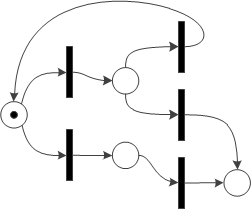
\includegraphics[scale=1]{include/AutomateNet.png}}
		\caption{Автоматная сеть.}
		\label{fig:fig1}
	\end{minipage}
	\hfill
	\begin{minipage}[H]{0.49\linewidth}
		\center{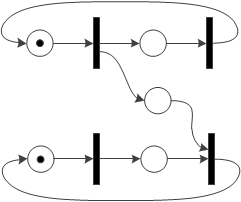
\includegraphics[scale=1]{include/SyncNet.png}}
		\caption{Синхронизационный граф.}
		\label{fig:fig2}
	\end{minipage}
\end{figure}
	
Простые сети Петри по выразительной мощности превосходят такие классы моделей, как конечные автоматы, но все же не все системы можно моделировать с их помощью. Это заставило искать такие обобщения сетей, которые увеличивали бы их выразительную мощность.

Это приводит к универсальным моделирующим системам, порождающим рекурсивно-перечислимые классы языков, т.е. к системам, равномощным машинам Тьюринга. Для дальнейшего исследования воспользуемся тем фактом, что машина Тьюринга равномощна счетчиковому автомату (модификация машины Минского). В \cite{Kotov} приводится доказательство того, что любой рекурсивно перечислимый язык порождается некоторым счетчиковым автоматом.

Счетчиковый автомат состоит из конечного множества счетчиков $ \{ x_{i} : 1 \leq i \leq N \} $, алфавита и программы автомата. Программа представляет из себя связный ориентированный граф с одной начальной вершиной без входных дуг, с одной заключительной вершиной без выходных дуг. Из остальных вершин выходит одна или две дуги. Вершинам приписаны операторы одного из шести типов:
\begin{enumerate}
\item начальной вершине приписан «старт», единственный в программе;
\item заключительной вершине приписан «стоп», единственный в программе;
\item оператор прибавления единицы $ x_{i} = x_{i} + 1 $, может быть приписан вершине с одной входной дугой;
\item оператор печати символа из алфавита автомата;
\item оператор недетерменированного перехода;
\item оператор условного вычитания единицы if $ x_{i} \neq 0 $ then $ x_{i} = x_{i} - 1 $.
\end{enumerate}

Все операторы, кроме условного вычитания единицы можно промоделировать с помощью сети Петри. Причина этого состоит в том, что в сети Петри можно заметить (отметить это срабатыванием некоторого перехода) тот факт, что место сети изменило разметку с нулевой на ненулевую, но нельзя отметить факт изменения разметки с ненулевой на нулевую. Таким образом из двух альтернатив ($ x_{i} \neq 0 $ и $ x_{i} = 0 $), содержащихся в операторе условного вычитания единицы, в сети Петри можно представить только первую, но нельзя отобразить проверку на ноль, т.к. сеть не может непосредственно среагировать на отсутствие фишки в месте (если место не ограничено).\cite{Piterson} Таким образом, для решения этих проблем вводится понятие ингибиторной сети (рис. \ref{fig:fig3}) и сети с приоритетами (\ref{fig:fig4}), которая строго мощнее класса сетей Петри. 

\begin{figure}
	\begin{minipage}[H]{0.49\linewidth}
		\center{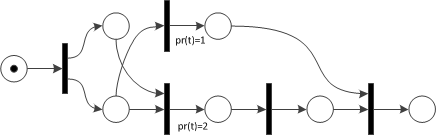
\includegraphics[scale=0.6]{include/PriorityNet.png}}
		\caption{Ингибиторная сеть.}
		\label{fig:fig3}
	\end{minipage}
	\hfill
	\begin{minipage}[H]{0.49\linewidth}
		\center{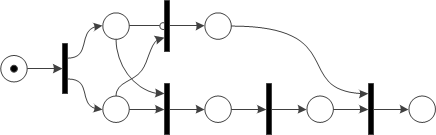
\includegraphics[scale=0.6]{include/IngibitorNet.png}}
		\caption{Сеть с приоритетами.}
		\label{fig:fig4}
	\end{minipage}
\end{figure}

При моделировании сетями Петри дискретных систем фишки часто соответствуют объектам, передаваемым от компонента к компоненту системы. Зачастую эти объекты имеют дополнительные атрибуты, позволяющие различать их и использовать эти различия для управления функционированием системы. Таким образом, мы приходим к модели сети Петри, в которой фишкам приписаны некоторые признаки, например цвет, а условие срабатывания переходов определяется таблицей, учитывающей цвета фишек. Такая сеть называется раскрашенной и является сетью, строго более мощной чем сеть Петри. Выразительная мощность раскрашенной сети Петри зависит от количества признаков. Класс сетей с конечным множеством признаком эквивалентен классу сетей Петри \cite{Kotov} \cite{Jensen}, хотя при преобразовании могут значительно увеличится размеры сети. 

Логичной модификацией сети Петри так же является разделение ее работы на такты. Такая сеть называется синхронной. В начале такта выясняется какие переходы могут сработать, из них выбирается максимальное множество взаимной неконфликтных переходов, затем это множество переходов срабатывает обычным образом меняя разметку сети. Необходимо отметить, что внутри такта выбранное множество срабатываемых переходов не меняется. Эта идея дает решение для проблемы недетерменированности переходов сети, т.е. для каждого перехода вводится его приоритет и порядок срабатывания определяется старшинством приоритетов. 

В сетях с приоритетами и синхронных сетях наметился отход от чисто локального принципа управления функционированием сети, принятого в сетях Петри, и переход к привлечению более глобальной информации о состоянии сети. Такой подход используется и в самомодифицирующихся сетях, в которых каждой дуге приписана модифицируемая кратность. Если кратность дуги ~--- число, то она имеет смысл, что и кратность в сетях Петри. Но в качестве кратности может выступать символ q некоторого места, в этом случае кратность дуги переменна и равна текущей разметке M(q) места q. Поскольку разметка места q может динамически меняться в процессе работы, то и кратность тех дуг, которым сопоставлен символ q, динамически меняется. Эта модификация интересна тем, что позволяет достаточно просто моделировать ингибиторные сети (рис. \ref{fig:fig5}) и сети с приоритетами (рис. \ref{fig:fig6}), т.е. сеть равномощна машине Тьюринга.

\begin{figure}
	\begin{minipage}[H]{0.49\linewidth}
		\center{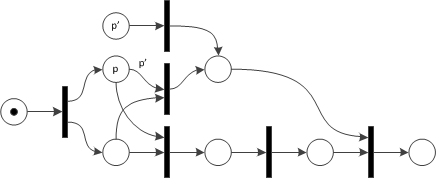
\includegraphics[scale=0.6]{include/SelfmodifiedNet1.png}}
		\caption{Самомодифицирующаяся сеть, эквивалентная ингибиторной сети на рис. \ref{fig:fig3}.}
		\label{fig:fig5}
	\end{minipage}
	\hfill
	\begin{minipage}[H]{0.49\linewidth}
		\center{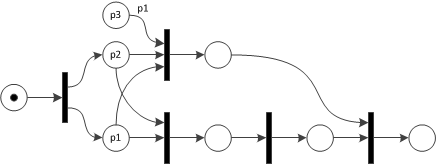
\includegraphics[scale=0.6]{include/SelfmodifiedNet2.png}}
		\caption{Самомодифицирующаяся сеть, эквивалентная сети с приоритетами на рис. \ref{fig:fig4}.}
		\label{fig:fig6}
	\end{minipage}
\end{figure}

Ниже в таблице \ref{tab:petri} приведено краткое сравнение выразительных мощностей модификаций сетей Петри. Типы сетей расположены в порядке возрастания их выразительной мощности.
\begin{center}
	\begin{longtable}{|p{0.05\textwidth}|p{0.2\textwidth}|p{0.7\textwidth}|}
		\caption{Сравнение выразительной мощности сетей.}
		\label{tab:petri}
		\\ \hline
		& Тип сети & Выразительная мощность
		\hline \endfirsthead
		\subcaption{Продолжение таблицы ~\ref{tab:petri}}
		\\ \hline \endhead
		\hline \subcaption{Продолжение на след. стр.}
		\endfoot
		\hline \endlastfoot
		1 & Автоматная сеть & Сохраняющая и дерево достижимости для нее является конечным. Из-за этого ограничения эта разновидность сетей неприменима для моделирования систем с разделяемым доступом. \\
		\hline
		2 & Обыкновенная сеть Петри & Используется для моделирования дискретных систем с разделяемым доступом. \\
		\hline
		3 & Раскрашенная сеть Петри & Такая модификация сети используется для упрощения сети за счет учета особенностей функционирования моделируемого объекта. Если множество признаком конечно, то сеть эквивалентна простой сети Петри. \\
		\hline
		4 & Ингибиторыне сети, сети с приоритетами и самомодифицирующиеся сети & Сеть описывает рекурсивно-перечислимые классы языков, равномощные машинам Тьюринга. В связи с этим в \cite{Piterson} формулируется теорема о том, что проблема ограниченности, достижимости, эквивалентности по префиксным и терминальным языкам, пустоты этих языков неразрешима для этих сетей \\
		\hline
		5 & Иерархические сети Петри & Иерархические сети являются обобщением регулярных сетей и служат для моделирования иерархических систем, которые на ряду с неделимыми, атомарными компонентами, содержат составные компоненты, сами представляющие собой систему. Иерархическая сеть функционирует, переходя от разметки к разметке, как и регулярная сеть, но правила функционирования иерархической сети отличаются от соответствующих правил для регулярной сети. Эти различия вызваны наличием составных переходов, срабатывание которых является не мгновенным событием, как в сетях Петри, а составными действием. \cite{Kotov} Иерархическая сеть обладает такими же моделирующими способностями, что и машина Тьюринга. \\
	\end{longtable}
\end{center}

\subsection{Раскрашенные сети Петри}

Теория раскрашенных сетей Петри разрабатывается более 20 лет рабочей группой (CPN Group) университета г.Орхуса (University of Aarhus, Denmark) под руководством профессора Курта Йенсена (Kurt Jensen). Этой группой разработана основная модель, включающая использование типов данных и иерархических конструкций, определены концепции динамических свойств, развивается теория методов анализа.

Раскрашенная сеть Петри ~--- это графоориентированный язык для проектирования, описания, имитации и контроля распределенных и параллельных систем. Графическими примитивами показывается течение процесса, а конструкциями специального языка имитируется необходимая обработка данных. Сеть представляет собой направленный граф с двумя типами вершин – позициями и переходами, при этом дуги не могут соединять вершины одного типа, т.е. граф является двудольным. Множество позиций (обозначаются эллипсом) описывают состояния системы. Переходы (обозначают прямоугольниками) описывают условия изменения состояний. Позиции называются входными для конкретного перехода, если направление дуги, указывает на переход. Позиции называются выходными для перехода, если дуга ведет от перехода к позиции.

В отличие от простых сетей Петри, в раскрашенных немаловажную роль играет типизация данных, основанная на понятии множества цветов, которое аналогично типу в декларативных языках программирования. Соответственно, для манипуляции цветом применяют переменные, функции и другие элементы, известные из языков программирования. Ключевой элемент сети ~--- позиция ~--- имеет определенное значение из множества цветов. \cite{Shahov}

Для отражения динамических свойств в сеть Петри введено понятие разметки сети, которая реализуется с помощью так называемых фишек, размещаемых в позициях. Цвет позиции определяет тип фишек, которые могут там находиться. Конкретизация фишки, находящейся в данной позиции, определяется инициализирующим выражением начальной разметки или формируется в результате правильного выполнения шага итерации сети Петри.

Сеть представляет собой асинхронную систему, в которой фишки перемещаются по позициям через переходы. Переход может сработать (т.е. переместить фишку из входной позиции в выходную для данного перехода), если во всех входных позициях для данного перехода присутствует хотя бы одна фишка и выполнено логическое выражение, ограничивающее переход (спусковая функция).

Дуги могут иметь пометки в виде выражений (переменных, констант или функций), определенных для множества цветов, и использоваться либо для «вычленения» компонентов сложного цвета фишек при определении условия срабатывания перехода, либо для изменения цвета фишки следующей позиции после срабатывания перехода. \cite{Kristensen}

\section{Анализ сетей Петри}

С помощью Сетей Петри можно моделировать широкий класс систем, представляя должным образом взаимодействие различных процессов. Наиболее мощны сети Петри в моделировании систем, включающих параллельные действия, причем параллельность моделируется естественным образом. Однако одно моделирование малополезно, необходимо провести анализ моделируемой системы. Для анализа используются два подхода: дерево достижимости и матричный метод.

В ходе анализа рассматриваются вопросы безопастности, ограничености, сохранения, активности и достижимости в сети.
\subsection*{Безопасность и ограниченость}
Сеть является ограниченой, если число фишек в каждой позиции не превышает N. Безопастность ~--- это частный случай ограничености. Безопастность позволяет представить позицию триггером, но в более общем случае можно использовать счетчик. Однако любой аппаратно-реализованный счетчик ограничен по максимальному числу, которое он может представить.

Позиция $ p_{i} \epsilon P $ сети Петри $ C = (P, T, I, O) $ с начальной маркировкой $ \mu $ является k-безопасной, если $ \mu'(p_{i}) \leqslant k $ для всех $ \mu' \epsilon R(C, \mu) $.

\subsection*{Сохранение}
Сеть является сохраняющей, если общее число фишек в системе не изменяется. Данное условие крайне важно в случае, если фишки представляют собой некоторые системные ресурсы.

\subsection*{Активность}
Сеть Петри является активной, если в ней не могут возникнуть тупики. Тупик в сети Петри ~--- это переход (множество переходов), которые не могут быть запущены. Переход называется активным, если он не тупиковый. Существует пять уровней активности:
\begin{enumerate}
\item Переход $ t_{i} $ обладает \textbf{\textit{активностью уровня 0}}, если он никогда не может быть запущен.
\item Переход $ t_{i} $ обладает \textbf{\textit{активностью уровня 1}}, если он потенциально запустим, т.е. существует такая $ \mu' \epsilon R(C, \mu) $, что $ t_{i} $ разрешен в $ \mu' $ .
\item Переход $ t_{i} $ обладает \textbf{\textit{активностью уровня 2}}, если для всякого целого n существует последовательность запусков, в которых $ t_{i} $ присутствует по крайней мере n раз.
\item Переход $ t_{i} $ обладает \textbf{\textit{активностью уровня 3}}, если существует бесконечная последоватлеьность запусков, в которых t_{i} присутствует неограничено часто.
\item Переход $ t_{i} $ обладает \textbf{\textit{активностью уровня 4}}, если для всякой $ \mu' \epsilon R(C, \mu) $ существует такая последовательность запусков $\sigma $, что $ t_{i} $ разрешен в $ \delta(\mu', \sigma) $.
\end{enumerate}

Переход, обладающий активность уровня 0 называется пассивным. Переход, обладающий активностью уровня 4 называется активным.

\subsection*{Достижимость}
Для данной сети Петри C с маркировкой $ \mu $ определить $ \mu' \epsilon R(C, \mu) $. Это основаная задача анализа сетей, т.к. остальные задачи сводятся к задаче достижимости.

\subsection{Дерево достижимости}

Дерево достижимости представляет множество достижимости Сети Петри. Каждая i-я вершина дерева связывается с расширенной разметкой $ \mu(i) $. В расширенной разметке число меток в позиции может быть либо неотрицательным целым, либо бесконечно большим. Бесконечное число меток обозначим символом $ \omega $. Каждая вершина классифицируется или как граничная, терминальная, дублирующая вершина, или как внутренняя. Граничными являются вершины, которые еще не обработаны алгоритмом. После обработки граничные вершины становятся либо терминальными, либо дублирующими, либо внутренними. Терминальные (пассивные) маркировки ~--- это маркировки в которых нет разрешенных переходов. Дублирующие маркировки ~--– это маркировки, ранее встречающиеся в ранее встречающиеся в дереве.

Дерево достижимости можно использовать для решения задач безопастности, ограничености и сохранения. Его нельзя использовать для решения задач достижимости и активности в общем случае. Решение этих задач ограничено существованием символа $ \omega $. Символ $ \omega $ означает потерю информации; конкретные количества фишек отбрасываются, учитывается только существование их большого числа. \cite{Piterson} Вместе с тем, в отдельных конкретных случаях дерево достижимости позволяет судить о свойствах достижимости и активности. Например, сеть, дерево достижимости которой содержит терминальную вершину, не активна. Аналогично искомая маркировка $ \mu $ в задаче достижимости может встретиться в дереве достижимости, что означает ее достижимость. Кроме того, если маркировка не покрывается некоторой вершиной дерева достижимости, то она недостижима.

\subsection{Матричный способ}

Второй подход к анализу сетей Петри основан на матричном представлении сетей Петри. Альтернативный по отношению к определению сети Петри в виде $ (P, T, I, O) $ является определение двух матриц $ D^{+} $ и $ D^{-} $, представляющих входную и выходную функцию. Каждая матрица имеет m сток (по одной на переход) и n столбцов (по одному на позицию).

Матричная форма эквивалентна стандартной форме, но позволяет дать определение в терминах векторов и матриц. Пусть $ e[j] $ ~--- m-вектор, содержащий нули везде, кроме j-ой компоненты. Переход $ t_{j} $ представляется m-вектором $ e[j] $. Переход в $ t_{j} $ в маркировке $ \mu $ разрешен, если $ \mu \geqslant e[j] * D^{-} $, а результат запуска перехода $ t_{j} $ в маркировке $ \mu $ записывается как:
\begin{equation}
\delta(\mu, t_{j}) = \mu - e[j] * D^{-} + e[j] * D^{+} = \mu + e[j] * (D^{+} - D^{-}) = \mu + e[j] * D,
\end{equation}

где $ D = D^{+} - D^{-} $ ~--- основная матрица изменений.

Марикровка $ \mu' $ достижима из маркировки $ \mu $, если существует последовательность (возможно, пустая) запусков переходов $ \sigma $, которая приводит из $ \mu' $ в $ \mu $. Следовательно, получаем, что $ \mu' $ достижима из $ \mu $, если 
\begin{equation}
\mu' = \mu + x * D
\label{F:F1}
\end{equation}
имеет решение в неотрицательных целых.

Матричный подход к анализу сетей Петри очень перспективен, но имеет некоторые трудности. Прежде всего, матрица D не полностью отражает структуру сети: переходы, имеющие как входы, так и выходы из одной позиции (петли), представляются соответствующими элементами матриц $ D^{+} $ и $ D^{-} $, но затем уничтожаются в матрице $ D = D^{+} - D^{-} $.

Основная проблема заключается в том, что решение уравнения \ref{F:F1} является необходимым для достижимости, но не достаточным.